\chapter{Related Work and Background}\label{chap:relatedWork}
In order to see which extent the research questions have been answered by existing work, a literature review has been conducted in this chapter. The sampling procedure of the literature for this review can be found in Chapter~\ref{chap:generalmethods}. This review is an extension from a previously written literature review in the IMT4205 Research Project Planning course. 

\section{Background: Room Scale Virtual Reality}
Before discussion and information around redirected walking can take place, it is first necessary to understand what room scale VR is. When it comes to virtual reality, there are two primary modes which are used: a seated mode and a room scale mode. A seated mode mainly makes use of full rotation tracking on all three axes, while the physical position of the user is not tracked. In room scale VR, both rotation and physical position are tracked. This tracking mode allows the user to move around in their physical space while maintaining a 1:1 ratio of movement and interaction with the virtual world using fully tracked controllers. Redirected walking functions within the room scale mode of VR as this is the only mode where redirection of physical movement is possible. 

\section{Redirected Walking, Detection Thresholds, Cybersickness and Presence}
Before reviewing the literature on distractors, it would be beneficial to first review the general topic of redirected walking. This section provides some background as well as relevant existing work within this area.

\subsection{Background: Redirected Walking}
The concept of redirected walking was originally presented by Razzaque et al.~\cite{razzaque2001redirected} as an alternative to real walking in virtual environments. The primary motivator behind its introduction was to optimise the usage of physical tracking space. This optimisation, in turn, allows for the development of virtual environments that are larger than the physical tracking space at what was considered a minimal increase in simulator sickness. 

Since its introduction, redirected walking has seen a fair amount of development as an area of research. One particularly important study was Steinicke et al.'s research, which formalised the concept of detection thresholds and introduced a taxonomy of redirected walking techniques~\cite{5072212}. As part of the taxonomy, they introduced the concept of three types of redirection gains:
\begin{itemize}
    \item Translation Gain
    \item Rotation Gain
    \item Curvature Gain
\end{itemize}

Translation gain is defined as a gain of translational movement in the virtual world compared to the real world. Rotation gain is defined as a gain of head rotation in the virtual world compared to the real world. These rotational gains are usually applied on the vertical axis. Finally, curvature gains are defined as a camera manipulation that constantly injects small changes in vertical angles as the user walks around. This injection allows the user to be redirected so they physically walk on a curve when it appears that they walk in a straight line virtually. Specifically for curvature gains, we define it as the ratio: $\frac{1}{r}$ where $r$ is the radius of the circular arc that the user is walking on. Some direct examples of how the three gains work could be as follows:
\begin{description}
    \item[Translation Gain of 2:] The user walks 5 meters in the real world but travels 10 meters virtually
    \item[Rotation Gain of 2:] The user rotates 180 degrees in the real world but rotates 360 degrees virtually
    \item[Curvature gain of 1 (radius = 1m):] The user has travelled on a quarter circle after $\frac{\pi}{2}$ meters in the real world while walking in a straight line virtually.
\end{description}

\begin{figure}[tbph]
    \centering
    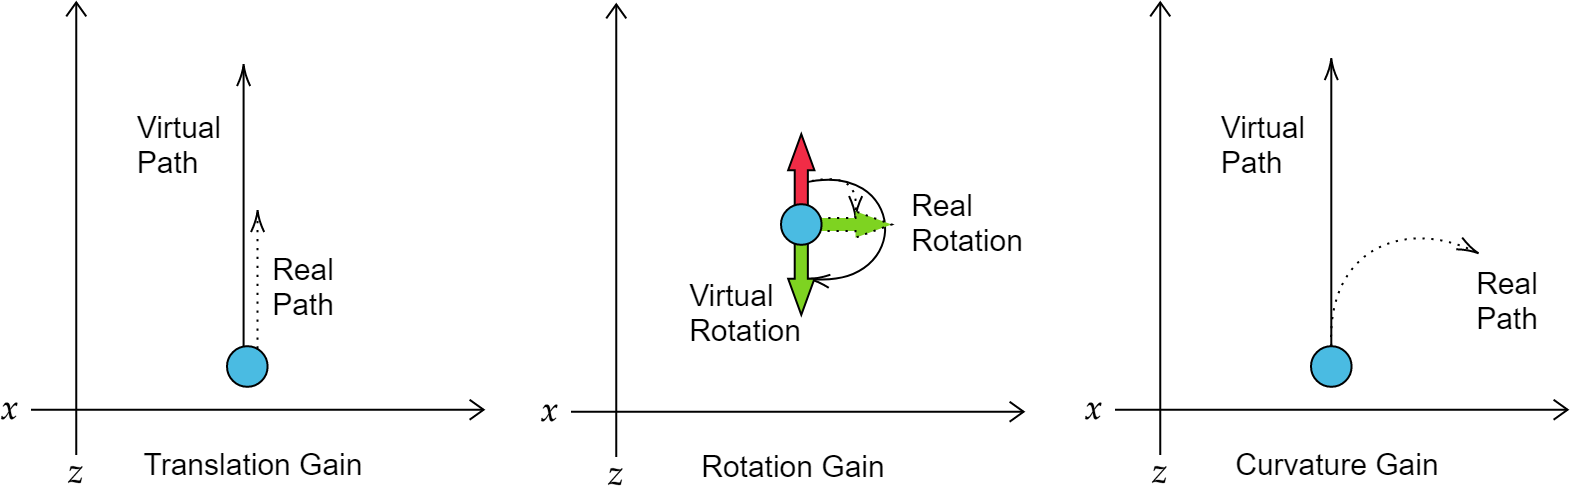
\includegraphics[width=1.0\textwidth]{figures/graphs/redirectionGains.png}
    \caption[Illustrated Example of How Redirection Gains Function]{This illustrated example shows how the three primary gains in redirected walking function.}
    \label{fig:redirectionGainsExample}
\end{figure}

Further illustration on how the different gains work can be seen in Figure~\ref{fig:redirectionGainsExample}.

Detection thresholds allow for the estimation of gains that can be applied without the user noticing them. As such, it has become a core of many other studies in the field. The taxonomy itself has since been extended by Suma et al.~\cite{suma2012taxonomy} to provide a more comprehensive look into additional redirection techniques. Outside of the three established redirection gains, an additional fourth type has recently been proposed by Langbehn et al.~\cite{7833190}. Their study presents the concept of bending gains which are similar to curvature gains but only applied whenever the user walks on a curve in the virtual world. 

In terms of relevance to research questions, the estimation of detection thresholds is directly relevant to $RQ_1$ as it provides a means to find undetectable gains. Despite this, there are some problems with this method of estimation that make it rather unsuitable to use. These are further mentioned in Section~\ref{sec:distractorUsageInLiterature}.

\subsection{Background: Redirection Algorithms}
In order to redirect a user, it is necessary to have a redirection algorithm. There are a variety of different redirection algorithms, but the two most common and generalised ones are as follows:
\begin{description}
    \item["Steer-to-Center"(S2C): ] A redirection algorithm that aims to steer the user towards the centre of the physical tracking space.
    \item["Steer-to-Orbit"(S2O): ] A redirection algorithm that aims to steer the user so they walk on the edge of a circle that encompasses the physical tracking space.
\end{description}
Both of these algorithms were originally presented by Razzaque~\cite{razzaque2005redirected} and have since been improved by Hodgson et al.~\cite{hodgson2013comparing}. The basis for these algorithms is to make use of rotation, curvature and translation gains in a manner that steers the user towards a desired point or direction. Among the two algorithms, S2C is generally believed to have the best performance, but S2O can perform better when long straight paths are travelled~\cite{hodgson2013comparing}. S2C has also been demonstrated to work particularly well for smaller physical spaces which is common for most virtual reality consumers today~\cite{azmandian2015physical}. 

Among the various redirection algorithms that exist, the most relevant for this thesis is Peck et al.'s "Improved Redirection with Distractors (IRD)"~\cite{peck2010improved}. This algorithm is an extension of the S2C algorithm with one primary addition: it makes use of virtual distractors to reorient the user towards the centre of the physical space when approaching physical walls. The usage of virtual distractors in redirected walking is further detailed in Section~\ref{sec:relatedDistractors}.

\subsection{Variables That Could Affect Redirected Walking and Detection Thresholds}
One thing to note about detection thresholds and the efficiency of redirected walking is that there are a variety of variables that can impact these. All the potential variables that were found throughout the sample of literature can be found in Table~\ref{table:DTVariables}. Since each variable is only briefly presented, there is a fair amount of abbreviated and potentially new terminology in use. The usage of abbreviated terminology will also increase from this point onwards in the thesis. As such, a short description of these can be found in Appendix~\ref{app:terminology} for quick referencing.

\begin{table}[!h]
\centering
\begin{tabularx}{\textwidth}{|m{2cm}|m{1.7cm}|m{10.1cm}|} 
\hline
Variable & Research Discussing Variable & Research Results|Comments in Parentheses\\
\hline
Size + Shape of Physical Tracking Space & 
\cite{azmandian2015physical} & 
There is no single ''optimal'' size.\newline Square shaped tracking spaces are the best choice for S2C and S2O algorithms.\newline S2C performs best in tracking spaces under 15m x 15m.\\
\hline
Optical Flow / Visual Density in VE & ~\cite{8446225, steinicke2008moving, 8446216, waldow2018textures} & Virtual environment size has no significant effect on detection thresholds.\newline It appears that low visual density/optical flow could make it harder to notice redirection.\newline Textures and global illumination have no significant effect on translation gain noticeability.\\
\hline
Hardware: HMD Field of View &
~\cite{fuglestad2018redirected}\newline Potentially relevant:\newline\cite{norouzi2018assessing} &
Detection thresholds for rotation and translation gain application are significantly lower with modern day hardware.\newline This could be caused by an increase in HMD field of view.\newline(This might correlate with increased optical flow).\\
\hline
Speed of Walking & \cite{5759454} & Likelihood of detecting curvature gains is significantly lower when walking slower.\newline Dynamic curvature gains allow for larger travel distances between resets compared to static gains.\\
\hline
Engagement / Distraction & \cite{5072212, schmitz2018you, sra2018vmotion}\newline Potentially relevant:\newline\cite{norouzi2018assessing, 5759454} & Whenever a user is engaged with a primary task or distracted by something, they appear to be less likely to notice that redirection is applied.\\
\hline
Awareness of Redirection & \cite{5072212} & If the user is not aware of the use of redirection, higher gains can be applied without being noticed.\\
\hline
Gender & \cite{nguyen2018individual} & Men seem to be more sensitive to curvature gains than women.\\
\hline
Adaptation: Curvature Gains & \cite{5072212, bolling2019shrinking, grechkin2016revisiting} & Exposing users to curvature gains for 20 minutes makes it harder to detect the gain. Similar effects might be possible for rotation, translation and bending gains. Gradually increasing the strength of curvature gains appears to cause some adaptation.\\
\hline
\end{tabularx}
\caption[Variables That Can Affect Detection Thresholds in Redirected Walking]{Variables that can affect detection thresholds in redirected walking.}
\label{table:DTVariables}
\end{table}

The variables that are found in Table~\ref{table:DTVariables} are relevant to this thesis as they can be used to inform the design of the virtual test environment, the use of redirection algorithms depending on available physical space and how to potentially maximise undetectable gains. Furthermore, the study by Azmandian et al.~\cite{azmandian2015physical} provides a means to measure the quality of redirection which is relevant for $RQ_2$.

\subsection{Comfort and Cybersickness}
While redirected walking aims at optimising the use of available tracking space and still leverage the benefits of real walking, it can result in some problems. High redirection gains tend to result in cybersickness, which can be seen as a form of motion sickness~\cite{mousavi2013review}. In doing so, one of the primary benefits of real walking is lost. Ideally, the increase in cybersickness from redirected walking should be minimised to provide the best user experience while still efficiently using the tracked space. In relation to detection thresholds, Fuglestad's research has shown that there might be an additional threshold between noticeable redirection and increases in cybersickness~\cite{fuglestad2018redirected}. These insights mean that it could be feasible to use estimated detection threshold values for redirection with limited risk of cybersickness increases, even if the user notices it at times. Similar results have been found by Rietzler et al.~\cite{rietzler2018rethinking}, suggesting that the use of curvature gains can be noticeable, but still acceptable. 

Outside of high redirection gains, there are also other factors that could increase cybersickness or limit user comfort. Dynamic field of view has for example been shown to potentially increase cybersickness~\cite{norouzi2018assessing}. Women might also be slightly more susceptible to cybersickness than men due to a slightly larger field of view~\cite{hildebrandt2018get}. Newer results from Nguyen et al. suggest otherwise though, as no significant increase in simulator sickness was found between genders in one of their experiments~\cite{nguyen2018individual}.

Due to the potential negative implications of standard redirected walking techniques, some researchers have developed new means of redirection. Suma et al. have made use of change blindness as a way to redirect without any type of gains~\cite{suma2011leveraging}. Despite this, their method only works for indoor environments and requires additional engineering for each individual room amongst these. Sra et al. have made use of scene rotation whenever the user is engaged with a task to leverage inattentional blindness~\cite{sra2018vmotion}, but their approach only works with predefined paths. 

From the point of view of a virtual environment designer, it would not be ideal to impose too many restrictions on how the environment is designed. At the same time, it is crucial to consider that cybersickness should be minimised as much as possible. Not doing so, can result in some ethical ramifications which are discussed in Section~\ref{sec:ethics}. For this thesis in particular, it is helpful to know that cybersickness can exist at a higher threshold than detection as this means that estimated gains could be possible to use safely. This knowledge has also been used to inform the method for estimating detection thresholds. 

\subsection{Subjective Sense of Presence}
Subjective sense of presence is a central part of virtual reality experiences. By properly immersing the user into a virtual world, it is possible to provide an engaging user experience. Subjective sense of presence can be negatively affected by a variety of techniques in redirected walking, which can compromise the overall experience of the user. 

The first of these are high redirection gains. Similar to Fuglestad's research that shows a difference between noticeability and cybersickness thresholds, Schmitz et al. presented that presence/immersion breaks at a different threshold from detection~\cite{schmitz2018you}. This insight means that certain gains of redirection can be noticed without resulting in cybersickness increases or breaks in presence.
Outside of redirection gains, another technique that can affect the subjective sense of presence is forced reorientation/resetting. Resetting techniques are fail-safes that are used whenever the user starts to exit the physical tracked space due to insufficient redirection~\cite{williams2007exploring}. An example of this would be to instruct the user to stop and rotate 360 degrees in the virtual world while they only rotate 180 degrees in reality due to applied rotational gains~\cite{suma2012taxonomy}. By doing so, the user is reoriented so that they no longer are in danger of leaving the tracked space. The problem with these types of techniques is that they are very intrusive and easily break any subjective sense of presence as the user has to temporarily stop what they were doing prior to resetting. 

Azmandian et al. mention that the average user should expect to have a physical tracking space that is 10m x 10m or lower, which results in many resets as unnoticeable redirection is not sufficient. Therefore they suggest that the focus should be on improving existing reset/reorientation mechanisms and better integrate them into the experience to limit breaks in presence~\cite{azmandian2015physical}. Improved subjective sense of presence and improved redirection are among the main areas that distractors aim to improve~\cite{peck2009evaluation, peck2011evaluation} which are the focus of this thesis.

\section{Distractors in Redirected Walking}\label{sec:relatedDistractors}
Distractors in redirected walking were originally presented by Peck et al. in 2009~\cite{peck2009evaluation}. In their study, the participants were instructed to watch a moving sphere and use this ''distraction'' as a means to increase redirection. Since then, various researchers have further improved distractors, although the term itself has acquired a few different semantic meanings. At the simplest level, a distractor when employed with redirected walking, aims to occupy the user's attention so that it is harder to notice redirection. As such, it is also possible to increase redirection during distraction~\cite{5072212}. This effect could potentially be a result of inattentional blindness which Sra et al. mention in their study on distractors~\cite{sra2018vmotion}. Distractors are triggered in a similar way to previous resetting/reorientation techniques(often shortened to "ROT", "ROTs" or simply resets), meaning that they activate whenever the user moves towards the edge of the physical tracking space. Compared to previous ROTs, distractors activate at a lower distance from the centre which means that existing ROTs can still be used as a fail-safe if the distractor itself fails to redirect the user~\cite{suma2012taxonomy}. Results from previous research also suggest that distractors result in higher levels of subjective presence compared to previous ROTs~\cite{peck2011evaluation}. 

From the acquired sample of literature, it does not seem like there is any formal taxonomy that defines the elements of distractors or their types. The closest to this would be Suma et al.'s taxonomy on redirection techniques~\cite{suma2012taxonomy}, but this taxonomy is too general to specify the details for distractors. As such, a grounded theory approach~\cite{strauss1994grounded} has been used to generate a taxonomy that classifies the most apparent elements that distractors consist of. This taxonomy will also be used as a framework to review the acquired sample of literature on distractors.

\subsection{Taxonomy of Distractors in Redirected Walking}\label{sec:distractorTaxonomy}
In cinematic VR, a similar topic to distractors is guided attention. While the goals behind a distractor and guided attention are somewhat different, there is some overlap that could be useful to consider. Taking inspiration from the taxonomy on redirected walking by Suma et al.~\cite{suma2012taxonomy}, Nielsen et al. have created a taxonomy of cues for guiding user attention in VR~\cite{nielsen2016missing}. Their taxonomy consists of three dimensions: explicit/implicit cues, diegetic/non-diegetic cues and whether they limit the ability to interact with the virtual environment (shortened to VE). Limiting interaction in the VE is not quite as relevant for redirected walking with distractors as physical walking is required, but the other two dimensions have been adapted into this taxonomy. The following sections describe general elements that can apply to any distractors, a distinction between two types of distractors and some elements that one of these can consist of. 
\subsubsection{Explicitness}
One of the relevant elements from Nielsen et al.'s taxonomy is explicitness. This element is split into explicit and implicit cues. An explicit cue consists of communicating that an event or object is deserving of attention while an implicit cue is meant to guide attention by simply being salient or interesting. In terms of distractors, these can also be explicit or implicit. An example of an explicit distractor would be a moving enemy in a VR game or something that the user has been told to pay attention to whenever it appears. As long as the user is told that they should pay attention to something, regardless of its purpose in the VE we can consider it as an explicit distractor. 

Implicit distractors on the other hand, would be distractors that can catch the user's attention in an almost instinctive manner. These could be salient elements that pop up in the peripheral vision of the user, potentially making them turn their head to see what it is. Another example would be a firefly that flies around and could catch the user's attention simply due to its salience in a darker environment. Compared to an explicit distractor like an enemy that the user knows they have to defeat, implicit distractors do not explicitly communicate how the user should react or interact with them. 

Currently, the usage of distractors is mostly of the explicit variety. A reason for this could be that the risk of ignoring an implicit distractor might be high. Unless the implicit distractor intrudes in a way that requires action from the user, it might not be seen as anything other than a detail in the scenery. The risk of ignoring a distractor can be problematic as there might not be enough redirection to avoid moving to the physical tracking boundaries. An effective implicit distractor might also be more challenging to design. It could be beneficial to have some background in psychology or neuroscience to understand what a natural user response would be to various implicit distractor scenarios.  

\subsubsection{Context Sensitivity}
An important aspect of distractors in the state of the art literature is context sensitivity~\cite{chen2017towards, chen2017supporting, sra2018vmotion}. Initial distractor implementations were fairly generic and worked similarly to standard ROTs, albeit with some changes. An example of this would be the hummingbird distractor from a study by Peck et al.~\cite{peck2011evaluation}. This distractor appears whenever the user approaches the physical boundaries and flies back and forth in front of the user. The user has in this case been instructed to keep their attention on the hummingbird, which then is exploited for redirection and reorientation. The downside of these generic types of distractors is that they serve no other purpose in the virtual experience other than to exploit the user for redirection and reorientation. This context insensitivity might not be ideal in terms of subjective sense of presence and can be seen as too repetitive if used too often in a short space of time. 

Instead, the focus with state of the art distractors has been to integrate them into the virtual experience so they serve additional purposes. VR games in particular are a good fit for integrating distractors as they can be included as game mechanics that are a central part of the experience. By doing so, there is less of a need for specialized instruction outside of understanding the premise of the game. There is also a belief by researchers that doing so will increase the subjective sense of presence~\cite{chen2017supporting, sra2018vmotion}. Improving the subjective sense of presence can be important considerations in the design of distractors as they could improve the user experience. 

Based on what has been seen in the literature, distractors could be categorised within four types of context sensitivity: Insensitive, Visually Integrated, Mechanically Integrated and Fully Integrated(Both visually and mechanically).

\subsubsection{Distractor Types}
The term ''distractor'' has primarily been used to describe objects in the VE that behave in a way that allows for redirection to be applied during distraction. A study by Sra et al.~\cite{sra2018vmotion} made use of distractor activities or simply ''attractors'' as they called it, which carries a slightly different semantic meaning. Due to this, it could be useful to differentiate between these two by splitting them into concrete and abstract categories.

\paragraph{Concrete Distractors}
If a distractor is an object or virtual existence in the VE, we can consider this as a concrete distractor. Concrete distractors consist of a variety of design elements which are further specified in the section following the description of abstract distractors. 

\paragraph{Abstract Distractors}
An activity on the other hand, can be considered as an abstract distractor. An activity can keep the user's attention by itself, but it can also consist of concrete distractors which require further attention of the user. If an abstract distractor is defined as an activity, then it is arguably explicit by nature as the user generally is aware of how they have to engage with it. An example of an abstract distractor would be to play a game, as various game elements and mechanics can keep the attention of the user. It does not matter what type of game the user plays as simply being engaged with it can be considered as a distraction, although its strength can of course vary. 

Abstract distractors can also be context sensitive or insensitive. An example of a context insensitive, abstract distractor would be to ask the user to perform a task that is entirely unrelated to what they are doing in the VE. An example of a context-sensitive, abstract distractor could be the activity of stargazing in an exploration-focused night-time scene. The activity of looking up into the sky could in this case allow for scene rotation while the user is looking upwards. The key to context sensitivity for these types of distractors is that they are believable and natural to the environment they are used in. 

\subsubsection{Elements of Concrete Distractors}
Concrete distractors can consist of a variety of elements that might result in specific user behaviour or to improve the user experience. The following paragraphs discuss the most apparent elements that were found by reading through the acquired sample of literature on distractors. This part of the taxonomy should be very easily extendable so that additional elements can be added in future work. 

\paragraph{Diegetic/Non-diegetic Existence}
The second element from Nielsen et al.'s framework regarding diegetic/non-diegetic cues is mostly relevant to concrete distractors. They define a diegetic cue as a cue that is a part of the world in the VE. By being part of the world, these cues are not only visible to one user, but also to any other users or computer controlled characters. An example of this would be to have a nearby volcano erupt. This event is then noticeable by both the players and any potential virtual characters in the narrative. A non-diegetic cue on the other hand, is only visible to one user. An example of this would be a HUD or GUI that only one user sees. To provide some examples within the scope of concrete distractors: a concrete, diegetic distractor could be a virtual character that the player interacts with while a concrete, non-diegetic distractor could be useful information in a HUD that the player wants to frequently keep attention on.

Diegetic cues could potentially improve the subjective sense of presence as Nielsen et al. achieved borderline significant results in their study~\cite{nielsen2016missing}. This insight could in turn also be relevant for concrete distractors. At the same time, in the context of games, it is not uncommon to have certain UI or elements that always are visible on the screen. If the game does not aim for realism, suspension of disbelief from the player could still result in a high subjective sense of presence. Due to this, one should not discredit the usage of distractors that are non-diegetic.

\paragraph{Movement}
Another element that concrete distractors consist of is movement or the lack of it. In terms of redirection, a concrete distractor can move around in a way makes the user turn their head. This movement can be used to apply rotational gains. An example of this would be a concrete distractor that orbits around the user and is important enough that they want to keep it in their vision at all times. If a concrete distractor moves towards the user, it might result in the user attempting to avoid it which can be used to move them away from physical walls or to apply redirection. A concrete distractor can also be useful for head-turning when static. An example would be to place a treasure chest at an angle from the user. In order to get the treasure, the user has to turn their head and move towards it which can be combined with rotation, curvature and translation gains.

\paragraph{First Appearance in Vision}
How the concrete distractor first appears in the user's vision is also something to consider. It could appear in plain sight, in the peripheral vision or outside of the user's vision. If a concrete distractor appears in the user's peripheral vision, it might catch their attention and make them turn their head to see what it is. If it appears outside of the user's vision, an audio cue or visual effects could be used to direct their attention towards where it is. If it appears in plain sight, the distractor might need to move around in order to apply rotational gains or to keep the user occupied so they do not notice a scene rotation. An example of this would be a merchant that allows the user to view their wares in a book or pamphlet. While the user is reading, the scene can rotate for the sake of redirection. 
         
\paragraph{Deterrents and Attractors}
Peck et al. introduced the concept of deterrents as a supplement to distractors~\cite{peck2011evaluation}. In their study, a deterrent was defined as something that deters the user from moving towards it. An example of a deterrent would be walls of fire that a fire-breathing dragon creates in Chen and Fuch's study~\cite{chen2017supporting}. In their study, these deterrents were used as a means to deter the user away from physical walls through strategic placement. Given that deterrents are capable of catching the user's attention, they could be seen as a type of concrete distractors. 

The opposite of a deterrent would be an attractor which the user wants to engage with. This definition is similar to Sra et al.'s definition of attractors~\cite{sra2018vmotion}, but instead of an activity, this definition is focused on concrete distractors. One of the previous examples of a treasure chest appearing at an angle that forces redirection could also be considered as an attractor. 

\paragraph{Salience}
The final element of concrete distractors is salience. Salience is defined as how easily a visual object stands out from its surroundings. In terms of distractors, salience can be important so that the user can quickly identify and place their attention on any concrete distractors that are used. An example of salient things that are effective at drawing attention could be moving objects or moving lights~\cite{rothe2018guiding}. 
Visual salience is comprehensive enough to be its own topic, although Nielsen et al. have mentioned some central factors that are believed to influence salience~\cite{nielsen2016missing}:
\begin{itemize}
    \item Luminance Contrast
    \item Edge or Line Orientation
    \item Colour
    \item Motion
    \item Stereo Disparity
\end{itemize}
One thing to note about these factors is that it is also important to consider how they contrast with the surrounding environment. Furthermore, the distribution of salient regions in a scene has a significant impact on how the user explores it as seen in a study by Sitzmann et al.~\cite{sitzmann2018saliency}. Their findings show that having few salient regions in a scene results in attention being shifted faster towards anything salient. As an additional effect, this attention is also more concentrated. These insights have been considered in the design of the virtual experience that is used for Experiment 1 and 2 in this thesis.

\section{Usage of Distractors in the Literature}\label{sec:distractorUsageInLiterature}
The previously generated taxonomy has been used as a framework to map out the usage of distractors in the acquired sample of literature. This mapping can be found in Table~\ref{table:DistractorsInLiterature}.

\begin{sidewaystable}[p!]
\centering
\scalebox{0.8}{
\begin{tabularx}{\textwidth}{|m{2cm}|m{1.5cm}|m{2cm}|m{1.9cm}|m{2cm}|m{7.55cm}|} 
\hline
Distractor & Used in Study & Explicitness & Context Sensitivity & Distractor Type & Additional Relevant Elements\\
\hline
Floating Sphere & \cite{peck2009evaluation} & Explicit & Insensitive & Concrete & Non-diegetic, Has movement, Appears in front of user.\\
\hline
Butterfly & \cite{peck2009evaluation, norouzi2018assessing} & Explicit & Insensitive: \cite{peck2009evaluation},\newline Visually Integrated: \cite{norouzi2018assessing} & Concrete & Diegetic, Has Movement.\\
\hline
Ghost & \cite{peck2010improved} & Explicit & Visually\newline Integrated & Concrete & Diegetic, Has Movement, Appears in front of user.\\
\hline
Hummingbird & \cite{peck2011evaluation, suma2012taxonomy} & Explicit & Insensitive & Concrete & Diegetic, Has Movement, Appears in front of user.\\
\hline
Horizontal Bars & \cite{peck2011evaluation} & Implicit & Fully\newline Integrated & Concrete & Diegetic, Static, Fades into view as user nears physical walls, Used as a deterrent.\\
\hline
Temporary Objectives & \cite{grechkin2015towards} & Explicit & Undefined & Abstract & None.\\
\hline
Moving NPCs & \cite{5759454} & Implicit & Fully\newline Integrated & Concrete & Diegetic, Has movement, Moves into view from the side or walks in front of the user, Used as a deterrent.\\
\hline
Flying Dragon & \cite{chen2017towards, chen2017supporting} & Explicit & Fully\newline Integrated & Concrete & Diegetic, Has movement, Moves towards user from current position when active, Can be considered as a attractor.\\
\hline
Flame Walls & \cite{chen2017towards, chen2017supporting} & Implicit & Fully\newline Integrated & Concrete & Diegetic, Static, Spawned by dragon when near physical walls, Used as a deterrent.\\
\hline
Watching Exotic Birds & \cite{sra2018vmotion} & Explicit & Fully\newline Integrated & Abstract & The activity itself consists of concrete disctractors(birds). These birds move across the sky and have to be viewed through a pair of binoculars.\\
\hline
Observing Insects & \cite{sra2018vmotion} & Explicit & Fully\newline Integrated & Abstract & The activity itself consists of concrete disctractors(insects). Among the many insects, the user is asked to keep one of them in focus.\\
\hline
Observing Insect in a Piece of Amber & \cite{sra2018vmotion} & Explicit & Fully\newline Integrated & Abstract & The user has to hold a piece of amber towards the sky and rotate so they can find a viewing angle that allows them to see the insect inside.\\
\hline
Interacting with NPCs & \cite{sra2018vmotion} & Explicit & Fully\newline Integrated & Abstract & The user has to hold a conversation with a NPC which acts as a concrete distractor.\\
\hline
Playing a target shooting minigame & \cite{fuglestad2018redirected} & Explicit & Fully Integrated & Abstract & The targets that move around could be considered as concrete distractors. \\
\hline
\end{tabularx}}
\caption[Distractors in Literature, Framed Within ''The Taxonomy of Distractors in Redirected Walking'']{List of all distractors that were used in the sample of literature, framed within the ''The Taxonomy of Distractors in Redirected Walking''}
\label{table:DistractorsInLiterature}
\end{sidewaystable}
When looking at the current usage of distractors from the sample of literature, a few insights can be gained. Most distractors are explicit and the only instances that could be regarded as implicit were in cases of deterrents. Due to this, there are potentially unexplored areas when it comes to designing implicit distractors. As already mentioned in the description of the taxonomy, these can be rather challenging to design which is why we might not see them being used very often. Despite this, recent developments into redirected walking with eye tracking hardware makes use of techniques that closely resemble implicit distractors and could arguably be categorised among these. Some additional information on this can be found in the following section.

The vast majority of distractors in this review were also diegetic. This means that there is room to explore non-diegetic distractors that are integrated into the experience. Non-diegetic distractors could for example be used as aids for the user in games or scenarios where extra contextual information is helpful. 

Outside of the previously discussed elements, it should be noted that initial forms of distractors were mostly insensitive to context and could be seen as relatively generic. Over time, distractors have started to become more visually integrated with their respective virtual environments. The current state of the art has focused on fully integrating distractors by combining them with game mechanics and activities. Even so, the integration could go further as the currently developed prototypes are very simple. This thesis has aimed to develop a game prototype with a slightly broader scope than existing work and fully integrate it with distractors. The overall design space of fully integrated distractors is relatively large, which allows for additional exploration by researchers. There is not much documentation on the effectiveness of these types of distractors either, creating an opportunity for new research in the area~\cite{nilsson201815}. This thesis aims to provide some documentation on this through an experiment related to $RQ_2$.

The significant focus on context sensitivity in the field of distractors does create somewhat of a mismatch with the rigid structure of Steinicke et al.'s detection threshold estimation procedure~\cite{5072212} though. In particular, it becomes hard to create a virtual experience where distractors are fully integrated as the method for estimating detection thresholds would interfere too much with the possible design space of the experience. This issue is further coupled with some ethical problems which are discussed in Section~\ref{sec:ethics}. In the end, these issues makes it hard to justify using the standard procedure for estimating detection thresholds. As such, an alternative procedure is employed which is detailed in Section~\ref{sec:ex1EstimationMethod}. 

\section{Eye Tracking in Redirected Walking: A New Use Case For Distractors}\label{sec:relatedEyeTracking}
A sub-field within redirected walking that recently has seen some major development is the employment of eye tracking hardware to further redirect users. Sun et al. have created a redirection system that performs small redirections during eye saccades, which consist of a small moment of temporary blindness~\cite{sun2018towards}. Furthermore, they make use of a subtle gaze direction method which adds additional salience to nearby objects or elements in the environment that are in the peripheral vision. As a result, this implicitly encourages the eye to move towards these regions. This technique could very well be framed as using implicit distractors from the previously presented taxonomy and provides an interesting use case for distractors. By combining distractors with state of the art redirection methods that use eye tracking, it could be possible to further improve the potential strength of redirection. As distractors are aimed at keeping user attention, they would be very well fit to help with triggering eye saccades, particularly so if they move around. 

Outside of Sun et al.'s study, Langbehn et al. have introduced a similar technique that instead exploits eye blinks as a means to perform small redirections~\cite{langbehn2018blink}. As part of their suggestions for how to increase the amount of eye blinks a user makes, they suggested making use of bright lights or virtual objects that move towards the eye of the user. This suggestion could also be seen as a use case for distractors. As a result, if accurate and effective eye tracking hardware ends up becoming more common in the future, we might see distractors become an essential building block of future redirection techniques with this technology. 

For this thesis, making use of eye tracking hardware is outside of the scope. There are a few reasons for this. First of all, while VR eye tracking hardware is available for experimentation at campus, the accuracy of the tracking drops during moderately fast head turns. This accuracy issue is problematic when using distractors as they may result in this sort of behaviour. The reason for this accuracy drop in general is that the eye tracking hardware is calibrated with the assumption that the HMD stays static on the user's head. If a user then moves their head so the HMD receives even a tiny displacement in its position, the calibration starts to become inaccurate. This displacement could for example pose a problem for detecting eye saccades, while this would likely be less of an issue for detecting eye blinks. 

Outside of potential inaccuracy problems, learning to use eye tracking hardware also requires a fair amount of time. In order to include this technology within the thesis scope, it would have been preferable to learn to work with the hardware beforehand. Given how the hardware was just recently acquired, this was not possible.

\section{External Validity of Estimated Detection Thresholds}
Given the number of variables that potentially could affect detection thresholds, it would be difficult to think of these as generalised thresholds. For example, the thresholds that Steinicke et al. initially estimated were thought of as a worst case scenario due to the isolated nature of the study~\cite{5072212}. As such, they should be considered as a baseline while higher redirection is possible due to a variety of variables like engagement or distraction. Despite this, Fuglestad's results have shown that this baseline might be significantly lower than that of Steinicke et al.'s estimations due to the potential effect of better hardware~\cite{fuglestad2018redirected}. As such, one might start to wonder what role detection thresholds can fulfil as their generalisability is limited by many factors.  

Despite this limitation, there are still a variety of use cases that the estimation of detection thresholds could be applicable for. One of these would be as a tool to measure how much a variable can affect noticeability. By estimating baseline thresholds for a virtual experience and estimating a second group of thresholds whenever a variable is introduced or active, we can make direct comparisons in how the detection of redirection changes. As long as the context of the estimations is taken into account, detection thresholds can also provide a ballpark estimate for the expected amount of unnoticeable redirection. Given that similar contexts are employed by others, they should also receive similar results. If large volumes of detection thresholds were to be estimated across many different contexts and virtual environments, they might also help with providing an overview of the degrees which various variables can affect noticeability. 

This discussion is primarily relevant to $RQ_1$ and the estimation of detection thresholds. In particular, this research makes use of the first example when discussing use cases for detection thresholds where two groups of thresholds are estimated in one experiment. The first group consists of baseline detection thresholds for the virtual experience when no concrete distractors are active, while the second includes detection thresholds for when a concrete distractor is active. This approach allows for direct comparisons on how the introduction of concrete distractors changes the noticeability of redirection. This method of comparison does come with one caveat though. Estimating two groups of detection thresholds in the same amount of time as one would estimate one group results in lower accuracy. Despite this, as detection thresholds in general cannot be taken as entirely accurate due to the number of variables that can potentially affect the result, some error should be acceptable. 

\subsection{Use of Informed/Uninformed Participants For Redirection}
Among the various variables that can affect the noticeability of redirection, one that could need some additional discussion is the awareness of redirection. Steinicke et al. mention in their study on detection thresholds that it was possible to increase unnoticeable redirection when the user is unaware of it~\cite{5072212}. This unawareness has since been part of various experiments within redirected walking. For example, all the current state of the art studies on distractors did not inform their participants of redirection before the experiment~\cite{sra2018vmotion, chen2017towards, chen2017supporting}. While this can provide higher unnoticeable gains, one important question to think of is how applicable this would be in the real world. 

If we think of a real-world scenario where a successful application or game makes use of redirected walking, would it be realistic to assume that every single user is unaware of redirection? Since we live in a day and age where the internet keeps us connected, if some users discover the employment of redirection, this information can quickly spread to many others. This spread of knowledge could in turn result in the redirection becoming more easily noticeable. At the same time, Steinicke et al. also mention that being engaged in primary tasks or activities have a similar effect~\cite{5072212}. If a user then knows of the redirection but is engaged enough into the virtual experience, it might help to counteract the otherwise increased noticeability. Of course, it would not be realistic to assume that all users know that redirection is used either as reality would most likely be somewhere in-between. 
 
The challenge lies in trying to design experiments that are closer to what we would expect in the real world. Informing participants to some degree is for example necessary when estimating detection thresholds as they should understand when they should report a detection. If the detection threshold gains are then used in a second experiment to test the performance of redirection, using uninformed participants would not change any results as the gains stay static. As such, for this thesis in particular, it would make the most sense to keep participants informed on redirection for all experiments. This thesis tries to move towards a middle ground between fully informed and uninformed participants. Instead of explicitly mentioning every detail relating to what redirection techniques that are used, participants are mostly given a brief introduction to the topic. They are then asked to notify whenever they detect that the virtual experience feels inconsistent or sluggish. Furthermore, a small amount of deceit is used by mentioning a few additional quality metrics to limit potential priming effects. The information and consent sheet that is given to participants can be found in Appendix~\ref{app:informationconsent}.

An additional benefit of not making use of fully uninformed participants is that the potential sample broadens as some participants could be reused between experiments. As already mentioned in the previous section, it is vital to consider the context of the estimated detection thresholds when looking at the results. To help with this, the context relative to the currently established variables is summarised when presenting the results in Chapter~\ref{chap:ex1}. 

\section{Ethics of Estimating Detection Thresholds}\label{sec:ethics}
One problem with researching redirected walking is the ethics around potentially making participants cybersick. This can be particularly problematic when estimating detection thresholds with standard methods like Steinicke et al. have used~\cite{5072212}. Their method for estimating detection thresholds makes use of a two-alternative forced choice task with a uniform distribution of gains in a given range. These gains are then tested in random order where the participant has to answer whether the current gains are higher or lower than the norm. The problem with this approach is that this range of gains could have values that are high or low enough to result in cybersickness. As such, it could be considered to be unethical to estimate detection thresholds like this. Instead, this thesis makes use of an alternative method which is presented in Section~\ref{sec:ex1EstimationMethod}.

Another thing that should be noted is that all participants throughout the experiments in this thesis were told to stop the experiment at once if they experienced any cybersickness or nausea. While prematurely ending the experiment with a participant does not provide entirely accurate data, it can still hold some value for analysis. 
   
\section{Accessibility of Redirected Walking to Virtual Reality Developers}
If a developer is interested in or wants to test redirection techniques, they may be met with a relatively sizeable theoretical bar of entry. This bar of entry is mostly a result of the knowledge around redirected walking primarily being in the academic sphere with very few practical tutorials or code examples for how redirection techniques can be implemented. The possibility of having several key articles locked behind pay-walls does not help with this either. 

Despite this, there are some publicly available code repositories that can be looked at. A link to Fuglestad's implementation of various redirected walking elements in the Unreal Engine can for example be found in his masters thesis~\cite{fuglestad2018redirected}. Azmandian et al. have developed a redirected walking toolkit for the Unity Engine which consists of implementations for the S2C and S2O algorithms as well as some basic reset techniques~\cite{azmandian2016redirected}. It should be noted that this toolkit has not received any updates or additional features since its release in 2016. The work done with this thesis can verify that the toolkit is working with Unity's 2018.3 version.

The Redirected Walking Toolkit by Azmandian et al. is used as a base for implementation in this thesis. This choice is primarily a result of the author's preexisting familiarity with the Unity Engine, which allowed for a faster development process.

\section{Choosing an Sufficient Reset Technique}\label{sec:choosingTheRightReset}
One important thing to consider when developing a virtual reality experience that makes use of redirected walking is the reset technique that will be used. It should not be expected that redirection will be able to fully steer a user away from walls at all times, hence the necessity of these fail-safes. Regardless, there are quite a few different reset techniques available, potentially making it a challenge to choose the right one. 

There are three standard reset techniques which were initially presented by Williams et al.~\cite{williams2007exploring}:
\begin{description}
    \item["Freeze - Backup": ] The user is notified that they have reached the physical bounds and their virtual position is frozen. They are instructed to take steps backwards until the experience is unfrozen. 
    \item["Freeze - Turn": ] The user is notified that they have reached the physical bounds and the HMD display is frozen. They are instructed to turn 180 degrees, after which the display is unfrozen. 
    \item["2:1 - Turn": ] The user is notified that they have reached the physical bounds. They are instructed to turn 360 degrees virtually while a rotation gain of 2 is applied. This rotation results in a 360-degree turn in the virtual world and 180 in the real world.
\end{description}

Among these three, the 2:1 Turn technique is most commonly seen. This popularity could be due to its relative simplicity and what could be considered as a lower degree of intrusiveness compared to its alternatives. Freeze - Turn and Backup might also be seen as too jarring for users as they directly remove some control in terms of head and body movement in the virtual world.

While the 2:1 Turn technique is the most commonly used one, it does come with a few problems of its own. The high gain value of 2 could for example become uncomfortable for participants even if it only stays active for a short while. Another issue is that it is possible to become stuck between two adjacent sides of a room that are close to the corners. This issue is illustrated in Figure~\ref{fig:2to1turnProblem} and results in the user moving back and forth with resets happening in perpetual succession.  

\begin{figure}[htbp]
  \centering
  \includesvg{figures/svgs/2to1turn.svg}
  \caption[Potential Problem With 2:1 Turn Resetting]{A potential problem that can occur when using the 2:1 Turn resetting technique. The blue circle denotes the user. The red and green arrows indicate the facing direction before and after resetting. The shaded area is the bounds for triggering the reset technique.}
  \label{fig:2to1turnProblem}
\end{figure}

To deal with this problem, Nguyen et al. have provided two alternative resetting techniques~\cite{nguyen2018discrete}:

\begin{description}
   \item["To Center": ] This resetting technique tells the user to rotate 360 degrees virtually. A gain value is precomputed so that the facing direction of the user ends up towards the centre of the tracked space once the rotation is finished. As a result, the user rotates 360 degrees + an additional angle to offset them towards the centre of the tracked space.
   \item["To Corner": ] This reset technique works similarly to the "To Center" technique but instead targets the furthest corner in the room. 
\end{description}

These resetting techniques were shown to provide significantly less resets in total over the 2:1 Turn technique in a simulated scenario. Despite this, the authors did not consider an important practical problem that their resetting techniques can result in with current day HMD's. This problem is related to the physical tethering that most modern HMD's still use today. When rotating over 360 degrees in the real world, the tethered cable can easily get tangled and the user will need to avoid wrapping themselves in it. This wrapping is less of an issue for the 2:1 Turn reset as the user only rotates 180 degrees in the real world. 

To mitigate with the various problems and issues that current day resetting techniques consist of, this thesis has created a variation of the Freeze - Turn reset. This new reset, dubbed as ''Pause - Turn - Centre'' is detailed in Section~\ref{sec:pauseturncentre}.

\section{Overall Answers to Research Questions}
Since the generated taxonomy has partially operationalised various elements of distractors, it would be prudent to update the terminology of the research questions as well. 
The updated research questions are as follows: 
\begin{description}
   \item[$RQ_1$: ] How noticeable is redirected walking with fully integrated distractors in a playful virtual environment?
   \item[$RQ_2$: ] Given the highest unnoticeable gains, how effective is redirected walking with fully integrated distractors in a playful virtual environment?
\end{description}

The following two paragraphs summarise how the related work is relevant to the research questions.

\paragraph{$RQ_1$}
For the first research question, a variety of variables that can affect detection thresholds in redirected walking have been mentioned. These have been considered when designing the experiment and corresponding virtual experience. By focusing on an engaging experience designed around fully integrated distractors, it might be harder to notice the redirection, which in turn could allow for stronger gains. A method for measuring detection thresholds has also been provided by Steinicke et al.~\cite{5072212}, but it is not used due to problems related to ethics and generally not working well with the theme of fully integrated distractors. The current state of the art is focused on fully integrated distractors and the literature sample provided no research measuring detection thresholds for these. As such, measuring the detection thresholds for fully integrated distractors should be a reasonable contribution to the field of distractors in redirected walking.

\paragraph{$RQ_2$}
Azmandian et al. have provided a method to measure the effectiveness of redirection by recording the total number of forced reorientations using standard reset techniques~\cite{azmandian2015physical}. Since standard reset techniques can be included as fail-safes for distractors, this is relevant to make use of for this thesis. Furthermore, it also allows for comparison with a control condition to find the relative increase in effectiveness.

Breaks in presence and cybersickness are thresholds that can exist at higher gains than detection. Due to this, it would be reasonable to focus on the highest unnoticeable gains as the risk of negative impact on the experience for participants should be minimal. 

\section{Usage of Distractors in Other VR Research Fields}
While distractors are just one sub-field of redirected walking, there are similar concepts used in other VR research fields as well. One of the already mentioned ones is using cues in cinematic VR as a means to guide the attention of the user towards areas of interest during watching~\cite{nielsen2016missing}. Another area where we can see the usage of distractors is in the medical field where they are used for pain relief~\cite{malloy2010effectiveness, knight2018virtual}. In this field, abstract distractors are used as a means to reduce the pain that patients experience under burn injury care or to reduce experimental pain~\cite{malloy2010effectiveness}. Furthermore, using VR distractions has shown to significantly decrease the amount of reactive pain behaviour in comparison to traditional distraction methods~\cite{knight2018virtual}. 

In general, we can see that the concept of distracting someone for either their own benefit or for entertainment can be employed in various ways in different fields of VR research.

\section{Background: Transformation Hierarchies in Game Engines}
As part of Chapter~\ref{chap:implementation}, there will be more technical implementation details on how the various redirected walking parts of the solution are implemented. In order to understand these technicalities as well as Azmandian et al.'s toolkit~\cite{azmandian2016redirected}, it is first necessary to provide some background on one important topic: Transformation hierarchies in game engines.

A transformation hierarchy in computer games is a relatively simple concept, but can result in rather complex behaviour. The gist of a transformation hierarchy is that objects or entities can be parented to each other. When parented, the child will no longer be positioned directly in world space, but rather relative to its parent. As such, if a parent moves, so will all of its corresponding children who may have individual relative positions within the hierarchy. This cascading effect does not only have to be in respect to position changes, but also scale and rotation. If we for example have a car object in a game with all the individual parts as children of a root node, then we can modify the position, rotation or scale of the root and it will propagate to each of the children. This way, we can rotate, re-position or scale the entire car by merely modifying the root node in the hierarchy.

\section{Background: The Redirected Walking Toolkit}
Since the implemented solution for this thesis makes use of the redirected walking toolkit~\cite{azmandian2016redirected} as a base, it is first necessary to at least have an overview of it. 

\subsection{How Redirected Walking is Implemented in the Toolkit}
An interesting side effect of transformation hierarchies is the perception of change for the child nodes. This effect is essential to how redirected walking is implemented in the redirected walking toolkit. To best illustrate this effect, it is easiest to provide an example. Consider that we have a parent: \textbf{''Redirection Root''} with two children \textbf{''Camera''} and \textbf{''Physical Space Representation''}. The camera can move around in the representation of physical space and both children will always be correctly mapped with each other, regardless of how the parent's transformation changes. As children, from their perceived point of view, they are consistent with each other due to how transformation hierarchies function. The interesting part becomes if we place our virtual world outside of hierarchy that the root governs, or rather have root and virtual world on the same hierarchical level. 

If we now rotate the redirection root, the children will have the perception that it is the virtual world itself that rotates, and not themselves. Despite what the children perceive, it is their redirection root parent that rotates and not the virtual world itself. This effect is the essence of how redirected walking is implemented in this case. Both curvature and rotation gains are implemented by injecting small amounts of rotation to the y-axis of the redirection root as the child camera moves and looks around. By doing so, it is possible to create the perceived effect that the child camera rotates more or less in the virtual world, compared to the real one. In a similar vein, it is possible to create curved paths. 

\subsection{Toolkit Terminology}
The toolkit uses slightly different semantics and terminology compared to what we could consider as the standard set by Steinicke et al.~\cite{5072212}. For the sake of consistency with the toolkit itself, this terminology will be used forwards in the thesis. The terminology that is different and their equivalents are as follows:

\subsubsection{Rotation Gains}
The toolkit does not semantically think of rotation gains as a multiplier to head movement, but rather as a percentage increase or decrease which are respectively named positive and negative rotation gains. For example: a rotation gain multiplier of 2, meaning that head rotations are twice as fast in the virtual world would be the equivalent to a positive rotation gain of 1. In this case, it is a 100\% increase over the base rotation. A multiplier of 0 would respectively be equivalent to a negative rotation gain of -1, meaning that the head no longer can rotate on the y-axis.

\subsubsection{Curvature Gains}
Instead of defining curvature gains as a ratio relative to the radius of the circular arc, the redirected walking toolkit defines curvature gains as curvature radius. In this case, a curvature radius of 5m means that the user's curved path will be on the edge of a circle that has a radius of 5m. 

\subsubsection{Forced Reorientation Techniques}
''Forced reorientation techniques''/''ROTs'' are generally either called by this semantic name or simply as ''resets''. There is no direct consistency in the literature regarding which one researchers use, but the toolkit uses ''resets'' as the term for forced reorientation techniques. 

\subsection{Toolkit Structure}
\begin{figure}[tbph]
    \centering
    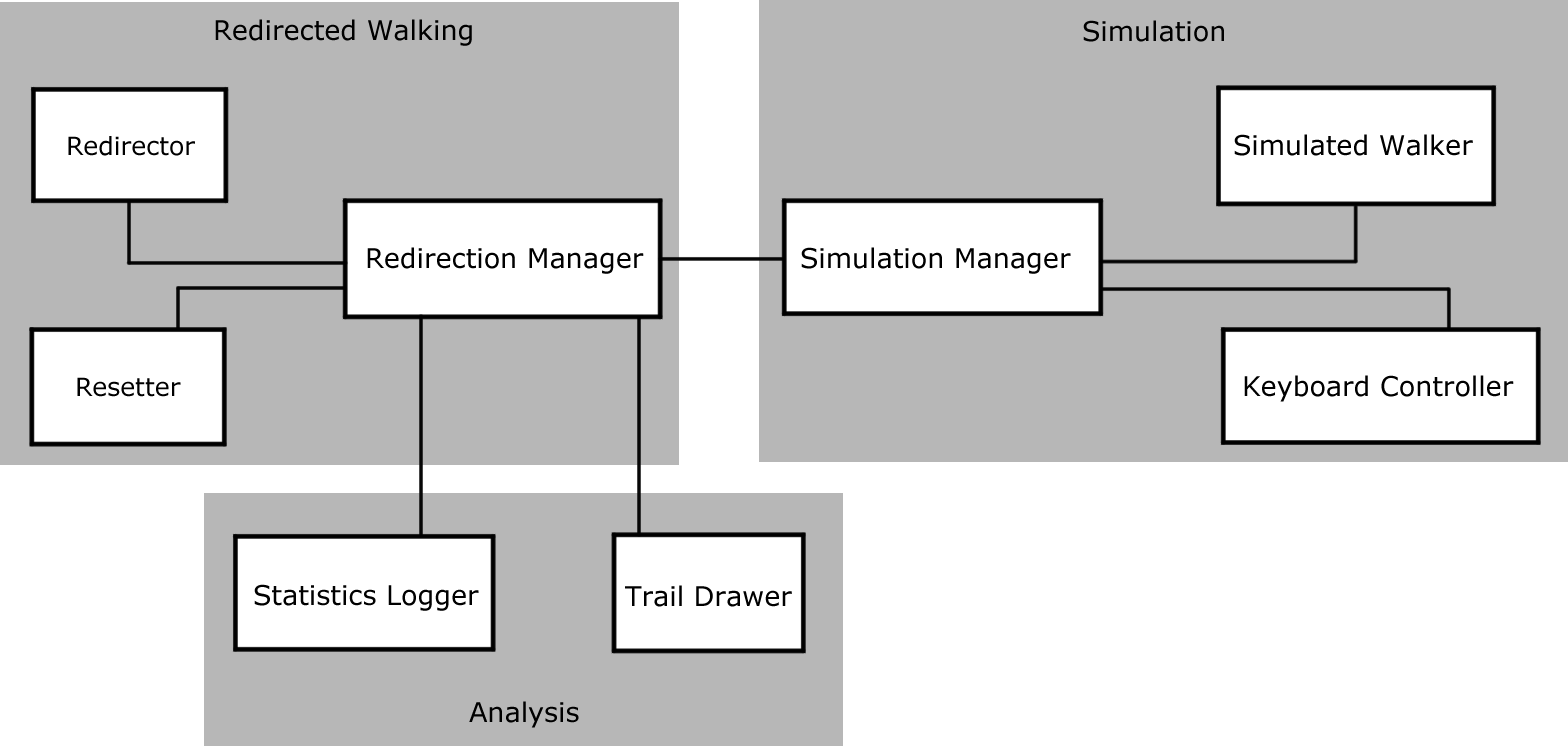
\includegraphics[width=1.0\textwidth]{figures/graphs/ToolkitStructure.png}
    \caption[Structure of the Redirected Walking Toolkit]{This illustration shows a recreation of Azmandian et al.'s figure~\cite{azmandian2016redirected} which gives an overview on the structure of the redirected walking toolkit. The structure has been further extended by the work in this thesis. The extended structure can be seen in Figure~\ref{fig:rdwToolkitExtendedStructure}.}
    \label{fig:rdwToolkitStructure}
\end{figure}

The redirected walking toolkit's overall structure is divided into three parts. These can be seen in Figure~\ref{fig:rdwToolkitStructure} and consist of redirected walking, simulation and analysis components. The work in this thesis is primarily related to the redirected walking side of the toolkit and as such, this part will be further detailed. 

\subsubsection{RedirectionManager}
The main control point of the toolkit is the \lstinline{RedirectionManager} script. The script itself is attached to the root object in the redirected walking object hierarchy and as the name implies, manages the whole solution. This management includes keeping track of the strength of gains, calling virtual functions on redirectors and resetters when applicable, and facilitating general communication between all of the components in the toolkit. 

\subsubsection{Redirectors}
Redirectors are the scripts in the toolkit that manage the injection of camera angles which results in redirection. All redirectors have to extend a base redirector script which makes use of various virtual functions that are called as necessary by the \lstinline{RedirectionManager}. The S2C and S2O redirectors are examples of scripts that in this case extend the base redirector class. This class allows for a generic approach where any type of redirector could be developed as long as it complies with the structure and virtual functions of the base class. 

\subsubsection{Resetters}
Resetters are similarly structured to redirectors. A resetter is capable of the same functionality as a redirector, but is only active whenever the user leaves a defined safe area within the physical space. By default, a resetter is triggered whenever the user is 0.5m away from the edge of the physical space. Furthermore, a resetter has additional callbacks for when a reset has triggered and when it is finished to allow developers to easily work with these events. 
